\documentclass{article}

%packages
\usepackage{graphicx}
\usepackage{tikz}
\usepackage[utf8]{inputenc}
\usepackage{amssymb}

\usepackage[T1]{fontenc}
\usepackage{mathabx}
\def\MCr{
	\multicolumn{1}{c}{
		\rule{-5pt}{0ex}$\stackrel{}{\curvearrowleft}$
		\rule{+20pt}{0ex}$\stackrel{}{\curvearrowright}$
	}
}
\def\MCe{\multicolumn{1}{c}{}}

\begin{document}

\usetikzlibrary{automata,arrows, positioning}
\renewcommand{\contentsname}{Tabla de contenidos}

\begin{titlepage}
	\begin{center}
		
\includegraphics{./images/escudo.jpg}
	\end{center}
	\centering
	{\scshape\LARGE Complutense de Madrid \par}
	\vspace{1cm}
	{\scshape\Large Práctica Programación Evolutiva.\par}
	\vspace{1.5cm}
	{\huge\bfseries Segunda práctica. \par}
	\vspace{2cm}
	{\Large\itshape Raúl Torrijos \& Lukas Häring\par}
	%{\large Grupo 9\par}
	\vfill
	\vfill

% Bottom of the page
	{\large \today\par}
\end{titlepage}

\tableofcontents

\newpage
\section{Introducción}
En está versión hemos implementado una modificación del Algoritmo Genético para aproximarnos a las posibles soluciones de El problema del viajante de comercio, utilizando mejoras sobre el esquema básico del Algoritmo Genético Simple.

\subsection{Mejoras implementadas}
Las mejoras implementadas sobre el AGS que hemos incluido en esta versión, y que por lo tanto no se encontraban implementadas en la Práctica 1 son:


\begin{enumerate}
	\item Algoritmos de Selección
		\begin{itemize}
			\item Selección por Ranking
			\item Selección por Truncamiento
		\end{itemize}
	\item Algoritmos de Cruce
		\begin{itemize}
			\item Emparejamiento Parcial (PMX)
			\item Cruce por Orden (OX)
			\item Cruce por Orden con posiciones prioritarias (OXPP)
			\item Cruce por Orden con orden prioritario (OXOP)
			\item Ciclos (CX)
			\item Recombinación de Rutas (ERX)
			\item Codificación Ordinal (CO)
			\item Método Propio 1 (explicado más adelante)
		\end{itemize}
	\item Algoritmos de Mutación
		\begin{itemize}
			\item Inserción
			\item Intercambio
			\item Inversión
			\item Heurística
			\item Método Propio 1 (explicado más adelante)
		\end{itemize}
	\item Otras mejoras
		\begin{itemize}
			\item Contractividad
			\item Mapa de España con el mejor recorrido representado gráficamente
		\end{itemize}

\end{enumerate}

\subsection{Aclaraciones}
Nos gustaría puntualizar un par de pequeñas decisiones que hemos tomado a la hora de implementar el ejercicio:\par
\bigskip
\quad- El número de ciudades que introducimos en el algoritmo es 27 (contando con Madrid), teniendo en cuenta que Madrid (id: 25) aparece tanto al principio como al final, nuestro cromosoma tiene por lo tanto 28 parámetros de entrada y cuenta con identificadores de ciudades desde el id: 0 (Albacete) hasta id: 26 (Málaga), por lo tanto nos dejamos fuera Murcia ya que entonces serían 28 ciudades y no 27.\par En cualquier caso nuestra implementación está preparada para ejecutar el problema con más o menos ciudades.\par
\bigskip
\quad- Hemos descubierto una errata en la tabla de distancias usada en la función de evaluación para evaluar el \emph{fitness} de las ciudades;  La distancia de \textbf{Guadalajara} a \textbf{Cuenca} es incorrecta, aparecen 486km cuando en realidad son 136km. Hemos actualizado al valor correcto en nuestra tabla. \par De este error nos hemos podido dar cuenta gracias a nuestra representación del mapa de España tras observar en reiteradas ocasiones que siempre trataba de evitar el camino entre estas ciudades.

\newpage

\section{Algoritmos Propios}

\subsection{Algoritmo de Cruce}
Nuestro algoritmo de cruza dos posibles soluciones al problema utilizando dos puntos de corte iguales en ambos padres y una componente aleatoria.
\begin{enumerate}
	\item Se generan dos enteros aleatorios que servirán como puntos de corte comunes para los padres.
	\item Se intercambian los subsegmentos entre los puntos.
	\item Para ambos hijos, se empieza desde la primera posición sin rellenar y se elige un candidato aleatoriamente.
	\item Si el gen elegido no está presente aún en el hijo, se inserta, si lo está se elige de nuevo un candidato aleatoriamente.
	\item Se repite el proceso para el otro hijo.
\end{enumerate}

\begin{tabular}{|l|*9{c|}}
	\MCe \\\hline
	Padre 1 & $a1_0$ & $a1_1$ & $\dots$ & $s1_{c1}$ & $\dots$ & $1s_{c2-1}$ & $\dots$ & $a1_{n-1}$ & $a1_{n}$ \\\hline
\end{tabular}

\begin{tabular}{|l|*9{c|}}
	\MCe \\\hline
	Padre 2 & $a2_0$ & $a2_1$ & $\dots$ & $s2_{c1}$ & $\dots$ & $s2_{c2-1}$ & $\dots$ & $a2_{n-1}$ & $a2_{n}$ \\\hline
\end{tabular}
\bigskip

\begin{tabular}{|l|*9{c|}}
	\MCe \\\hline
	Hijo 1 & $a1_0$ & $a1_1$ & $\dots$ & $s2_{c1}$ & $\dots$ & $s2_{c2-1}$ & $\dots$ & $a1_{n-1}$ & $a1_{n}$ \\\hline
\end{tabular}

\\
\begin{tabular}{|l|*9{c|}}
	\MCe \\\hline
	Hijo 2 & $a2_0$ & $a2_1$ & $\dots$ & $s1_{c1}$ & $\dots$ & $1s_{c2-1}$ & $\dots$ & $a2_{n-1}$ & $a2_{n}$ \\\hline
\end{tabular}
\newline\newline
Donde $c1, c2$ son los puntos de corte generados, $s1, s2$ los elementos de los subsegmentos a intercambiar, y $a1, a2$ los elementos generados aleatoriamente.
\newpage
\subsection{Algoritmo de Mutación}
El algoritmo consiste en evaluar dos posibles mutaciones, estas mutaciones son las que se producen al intercambiar alguno de los vecinos más cercanos.
Algoritmo:
\begin{enumerate}
	\item Se genera un entero aleatorio desde $2$ hasta $n-2$, donde n es la cantidad de genes.
	\item Se realiza un intercambio del elemento que apunta este puntero con el vecino de la izquierda.
	\item Si su evaluación es mejor, intercambiamos. Por el contrario, lo dejamos como está.
	\item Teniendo en cuenta el cromosoma sin modificar, realizamos un intercambio con el vecino de la derecha.
	\item De la misma forma, si la evaluación es mejor, intercambiamos.
\end{enumerate}
\newline

Como vemos, el número aleatorio se elige entre $2$ y $n-2$. Esto es, claro está, que si intercambiamos el puntero fuera $1$, este cogería como vecinos $0$ y $2$, haciendo que pudiera mutar el gen inicial (Y eso no debe ocurrir).


\begin{tabular}{|l|*7{c|}}
	\MCe & \MCe & \MCe & \MCe & \MCr & \MCe & \MCe \\\hline
	Cromosoma 1 & $a_0$ & $\dots$ & $a_{k-1}$ & $a_{k}$ & $a_{k-1}$ & $\dots$ & $a_{n}$ \\\hline
\end{tabular}
\newline\newline
Donde $k\in \{2, \dots, n-2\}\subseteq\mathbb{N}$

%subsection{Función 1}
%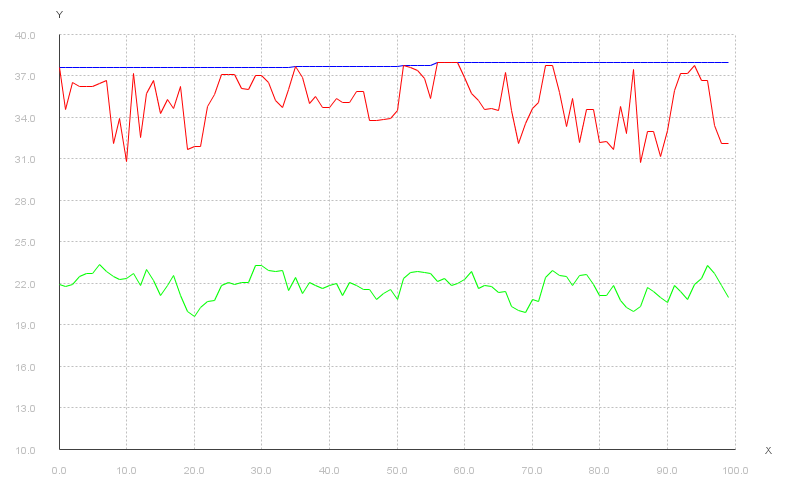
\includegraphics[scale=0.5]{./images/graph1_bin.png}
%En general, hemos observado que el grado de evolución global es mucho mayor cuando el elitismo está activado. La calidad media generacional se ve mejorada notablemente.

\newpage
\section{Análisis de ejecuciones}
Para realizar un análisis exhaustivo del comportamiento de cada uno de los algoritmos usados hemos realizado una gran cantidad de ejecuciones y hemos obtenido las siguientes conclusiones.
\subsection{Peores resultados}

Ruleta es el método de selección que menos favorece a la evolución ya que tiene una gran componente aleatoria y resuelve el ejercicio con valores muy lejanos al recorrido mínimo posible.
\\
\begin{figure}[h]
	\centering
	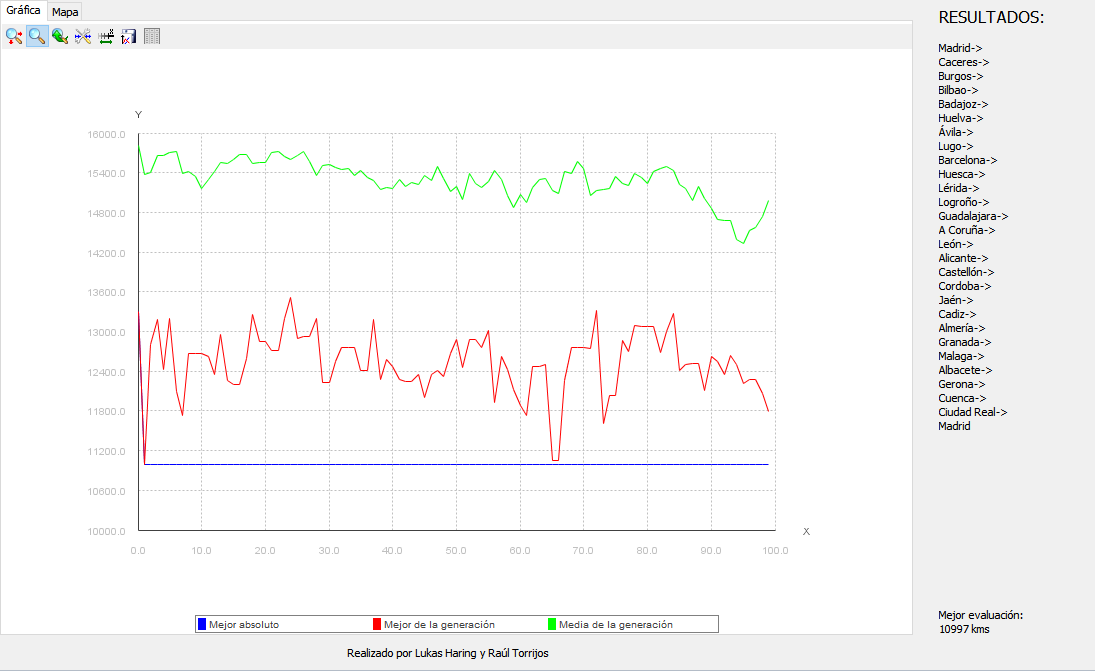
\includegraphics[scale=0.4]{./images/rule1.png}
	\caption{Ruleta sin contractividad ni elitismo}
\end{figure}



La única manera de obtener resultados mas razonables utilizando ruleta es usando contractividad y/o elitismo y/o ampliar el número de generaciones.


\begin{figure}[h]
	\centering
	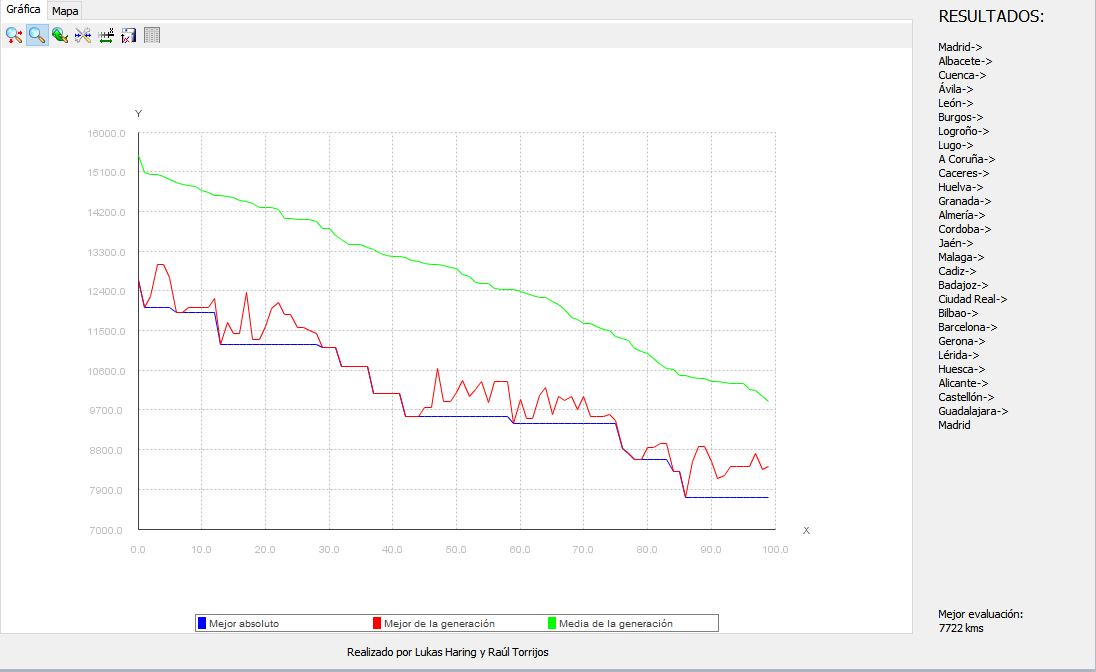
\includegraphics[scale=0.4]{./images/rule2.png}
	\caption{Ruleta con contractividad}
\end{figure}

\newpage
\subsection{Contractividad}
La contractividad hace que no pueda haber una generación con la media peor que la anterior, y esto en principio es algo positivo, pero puede suceder que cada vez sea más complicado sacar individuos mejores, y esto puede estancar el algoritmo\par Para ello es necesario añadir otra condición de salida además del número de generaciones y hemos optado por un criterio de terminación enfocado al coste, cuando se produzcan 1000 fallos seguidos al intentar conseguir una generación, para la ejecución
\\

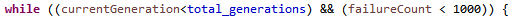
\includegraphics[scale=0.83]{./images/cont.png}

\subsection{Elitismo}
Hemos observado sobre este problema concreto el elitismo no adopta un papel demasiado determinante, ya que hemos conseguido valores muy próximos al recorrido mínimo posible sin elitismo activado
\newpage
\subsection{Mejores resultados}
Los mejores resultados que obtenemos son con Selección mediante Torneo Determinista, Cruce PMX o ERX, y con mutaciones mediante Inversión y Heurística.\par
En 50 ejecuciones hemos obtenido 17 veces el que consideramos el valor mínimo o \textbf{solución: 5155km}. También favorece aumentar el valor de individuos en nuestra población para aumentar las posibilidades de que obtenga el mínimo posible.
\begin{figure}[h]
	\centering
	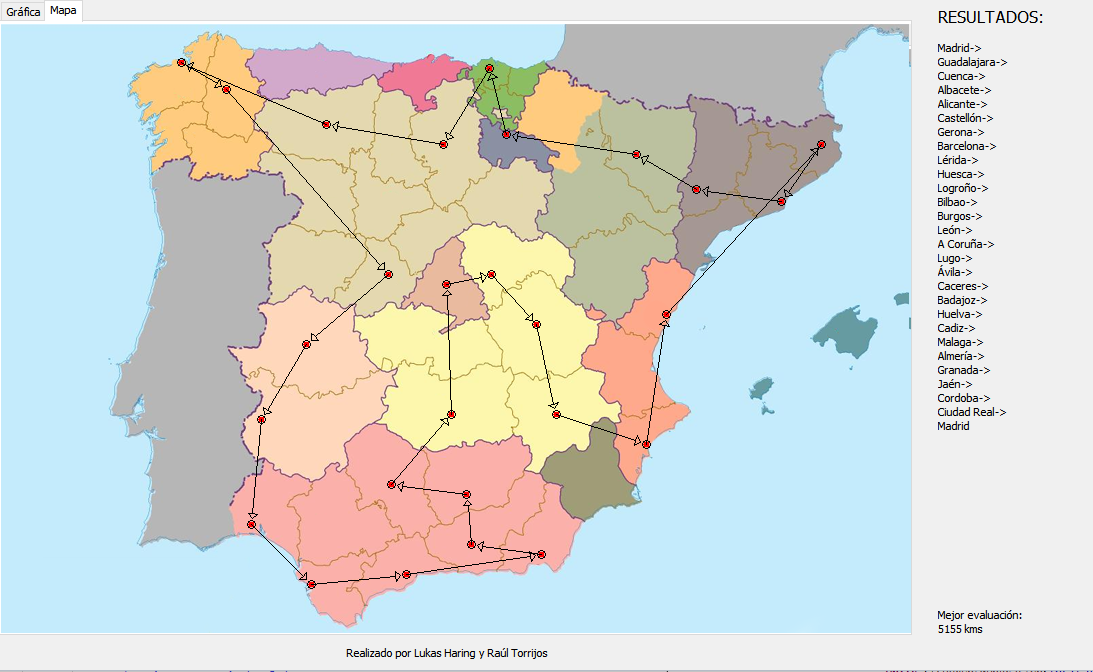
\includegraphics[scale=0.35]{./images/best.png}
	\caption{Representación geográfica. Mejor resultado obtenido. 5155km}
\end{figure}

\begin{figure}[h]
	\centering
	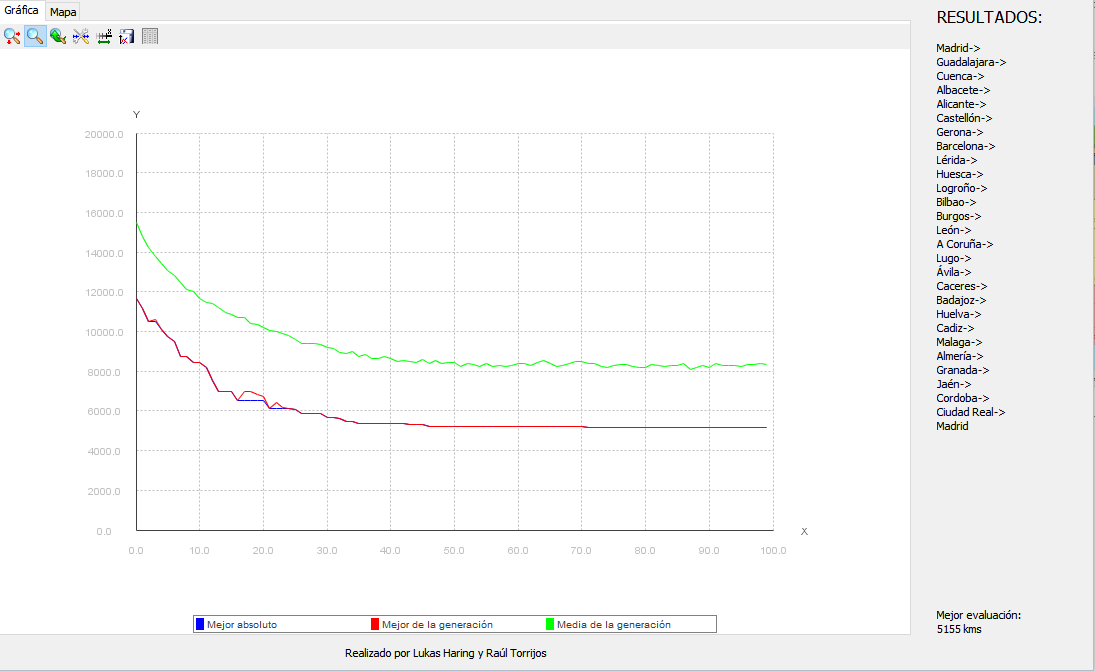
\includegraphics[scale=0.35]{./images/best2.png}
	\caption{Gráficas de evolución. Mejor resultado obtenido. 5155km}
\end{figure}
\end{document}
